
\section{Caminante Aleatorio}


\begin{frame}
	\frametitle{Caminante Aleatorio}
	\begin{figure}
		\centering
		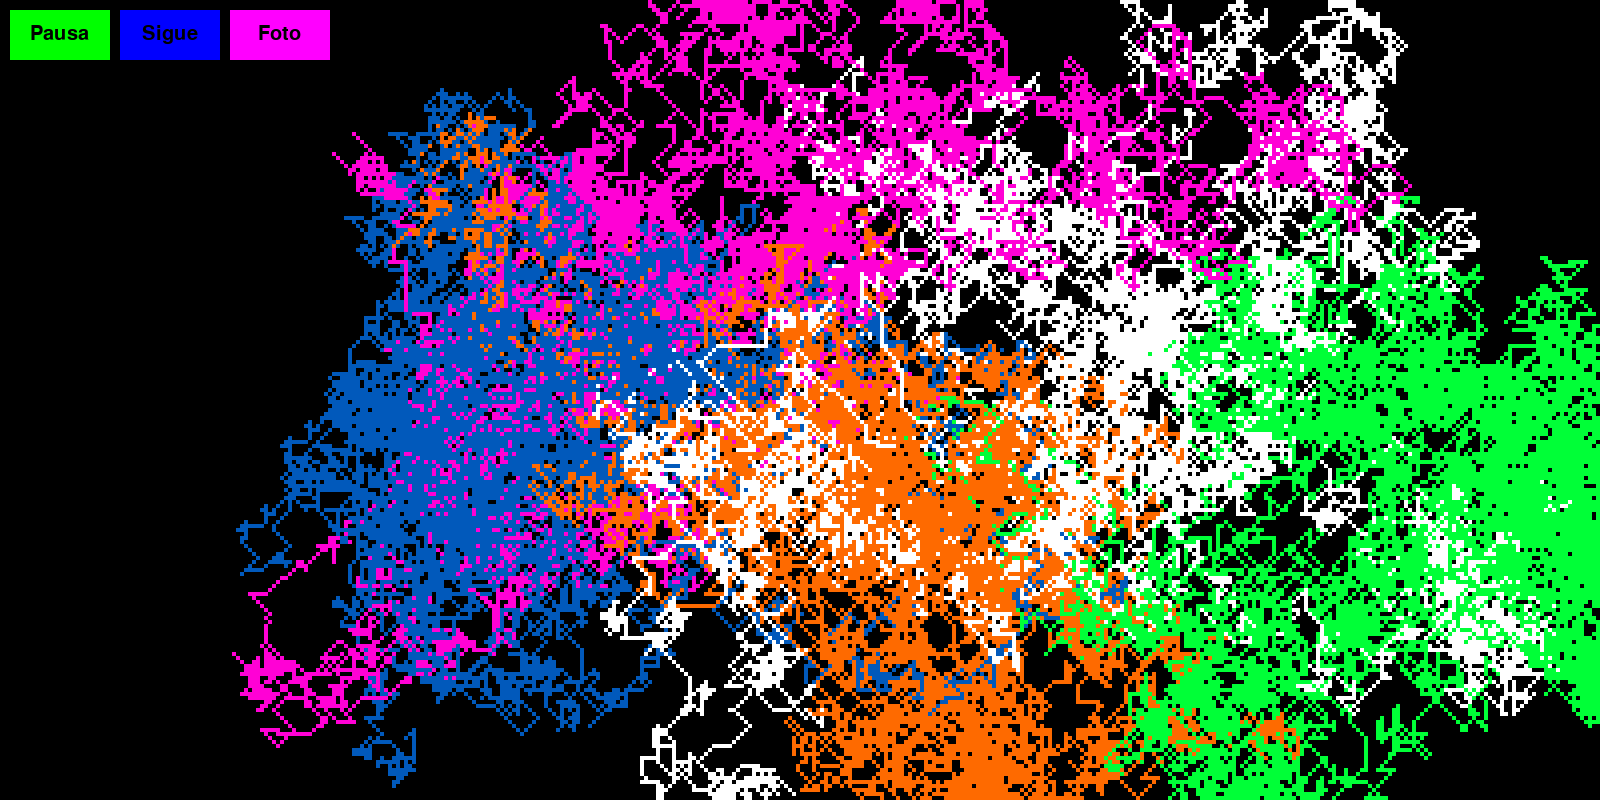
\includegraphics[width=\textwidth]{walkerUniforme} % Asegúrate de cambiar la ruta a la ubicación de tu imagen
		\caption{Caminante Aleatorio con distribución uniforme}
	\end{figure}
	
	
\end{frame}

\begin{frame}
	\frametitle{Caminante Aleatorio}
	Utilizando datos generados según distribuciones uniforme (\texttt{randomsUniforme.txt}), normal (\texttt{randomsNormal.txt}), y gamma (\texttt{randomsGamma.txt}), se propone crear una animación de caminante aleatorio. El objetivo es examinar cómo las diferentes distribuciones de probabilidad influyen en el comportamiento del caminante y en las series de tiempo derivadas. Se analizarán las siguientes métricas:
	
	\vspace{5mm}
	\begin{itemize}
		\item Dirección y distancia de cada paso.
		\item Incidencias de choques con obstáculos.
		\item Evolución de la posición (x,y) en el plano.
	\end{itemize}
	
\end{frame}


\begin{frame}
	\frametitle{Caminante Aleatorio - Datos Uniformes}
	\begin{figure}
		\centering
		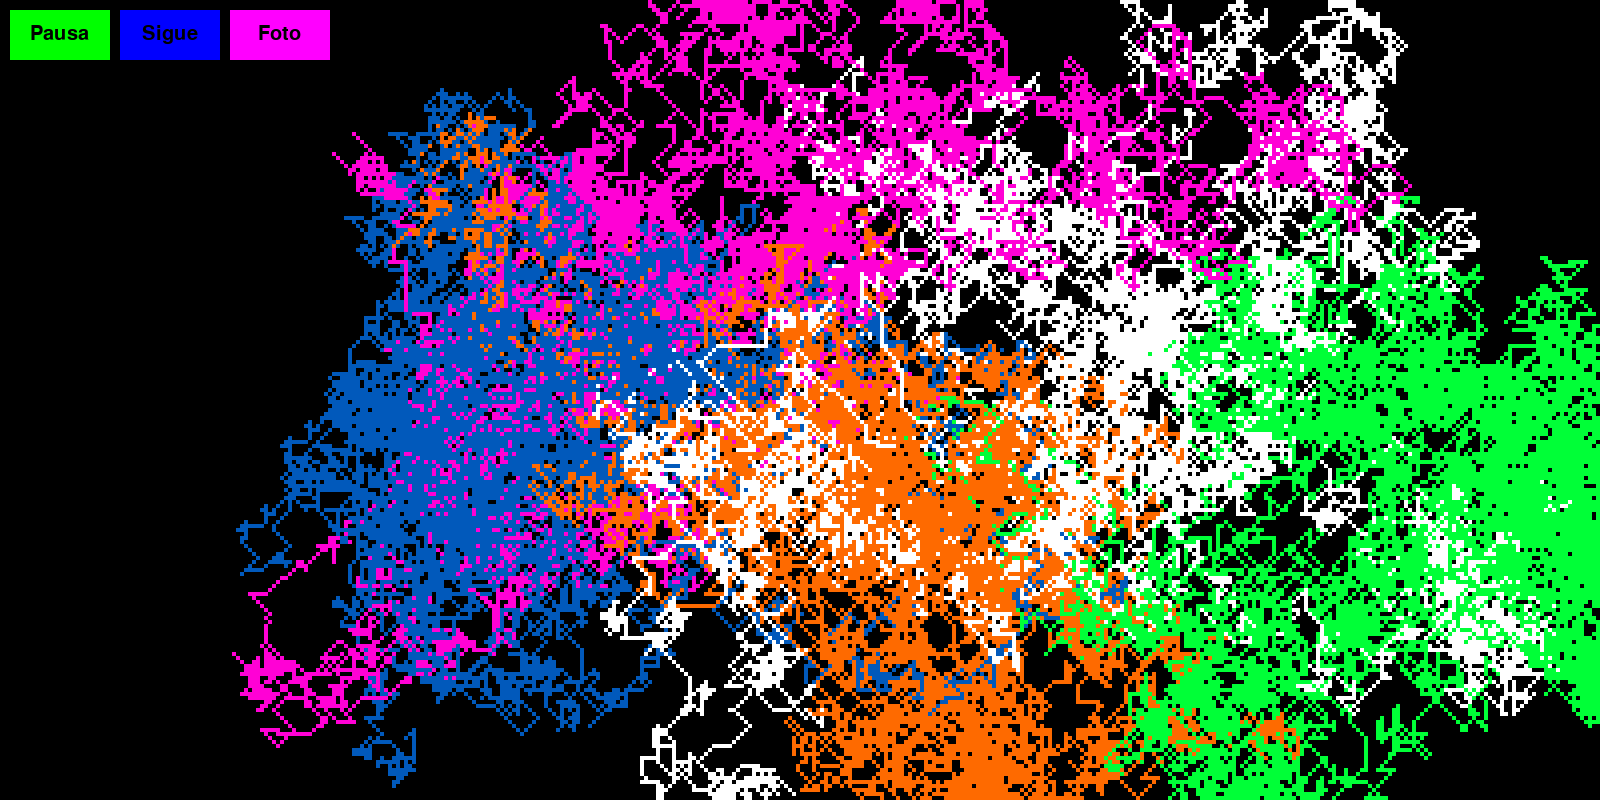
\includegraphics[width=\textwidth]{walkerUniforme} % Asegúrate de cambiar la ruta a la ubicación de tu imagen
		\caption{Caminante Aleatorio con distribución uniforme}
	\end{figure}
\end{frame}

\begin{frame}
	\frametitle{Gamma - Uniforme}
	
	\begin{columns}
		
		% Columna de la izquierda
		\begin{column}{0.5\textwidth} % Ajusta la proporción según necesites
			\begin{figure}
				\centering
				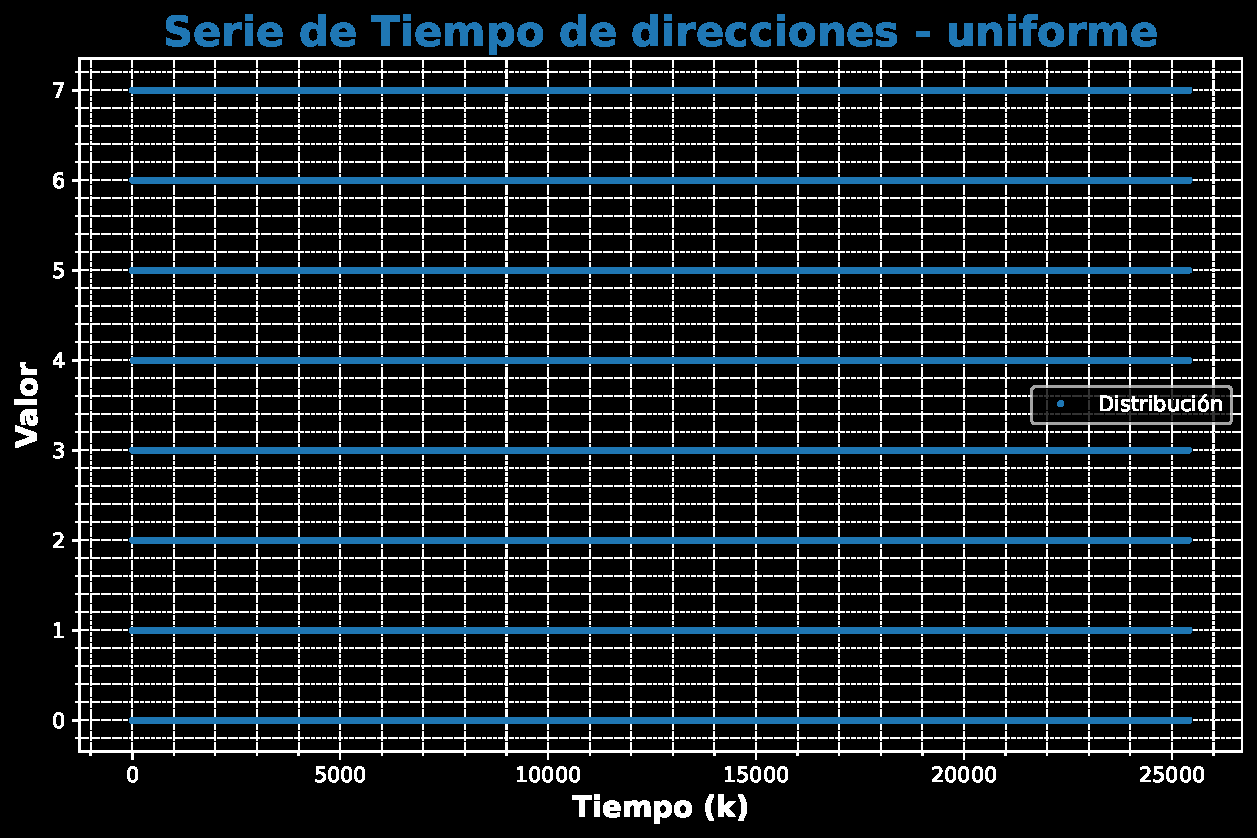
\includegraphics[width=\textwidth]{graf_direcciones_uniforme} % Asegúrate de cambiar la ruta a la ubicación de tu imagen
				\caption{Gráfica de la serie de tiempo para las direcciones.}
			\end{figure}
		\end{column}
		
		% Columna de la derecha
		\begin{column}{0.5\textwidth} % Ajusta la proporción según necesites
			\begin{figure}
				\centering
				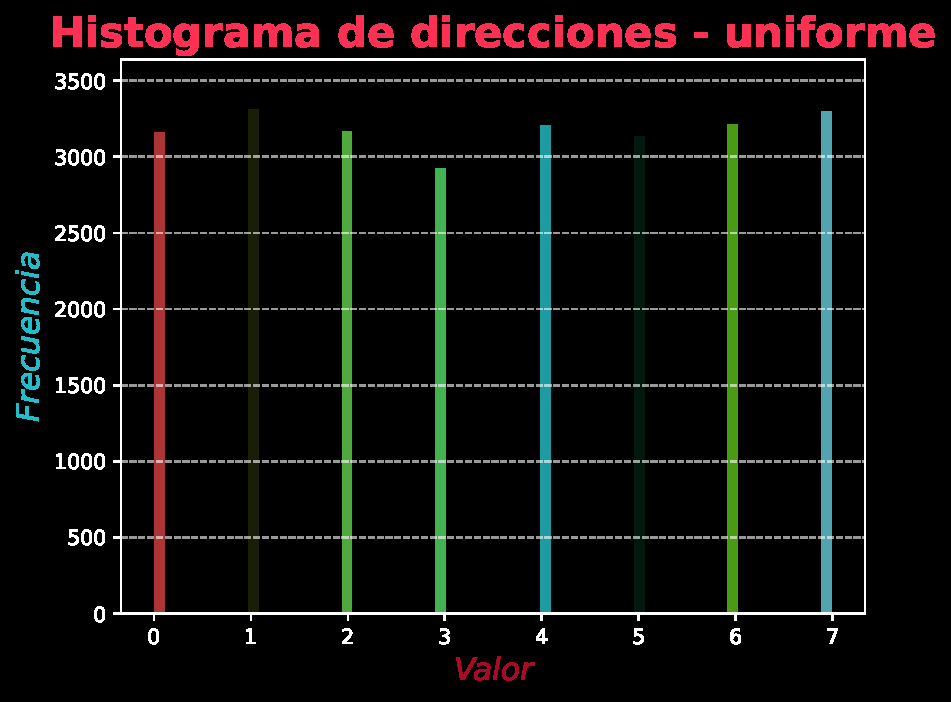
\includegraphics[width=\textwidth]{hist_direcciones_uniforme} % Asegúrate de cambiar la ruta a la ubicación de tu imagen
				\caption{Histograma de los datos de direcciones.}
			\end{figure}
		\end{column}
	\end{columns}
\end{frame}


\begin{frame}
	\frametitle{Caminante Aleatorio - Datos Normal}
	\begin{figure}
		\centering
		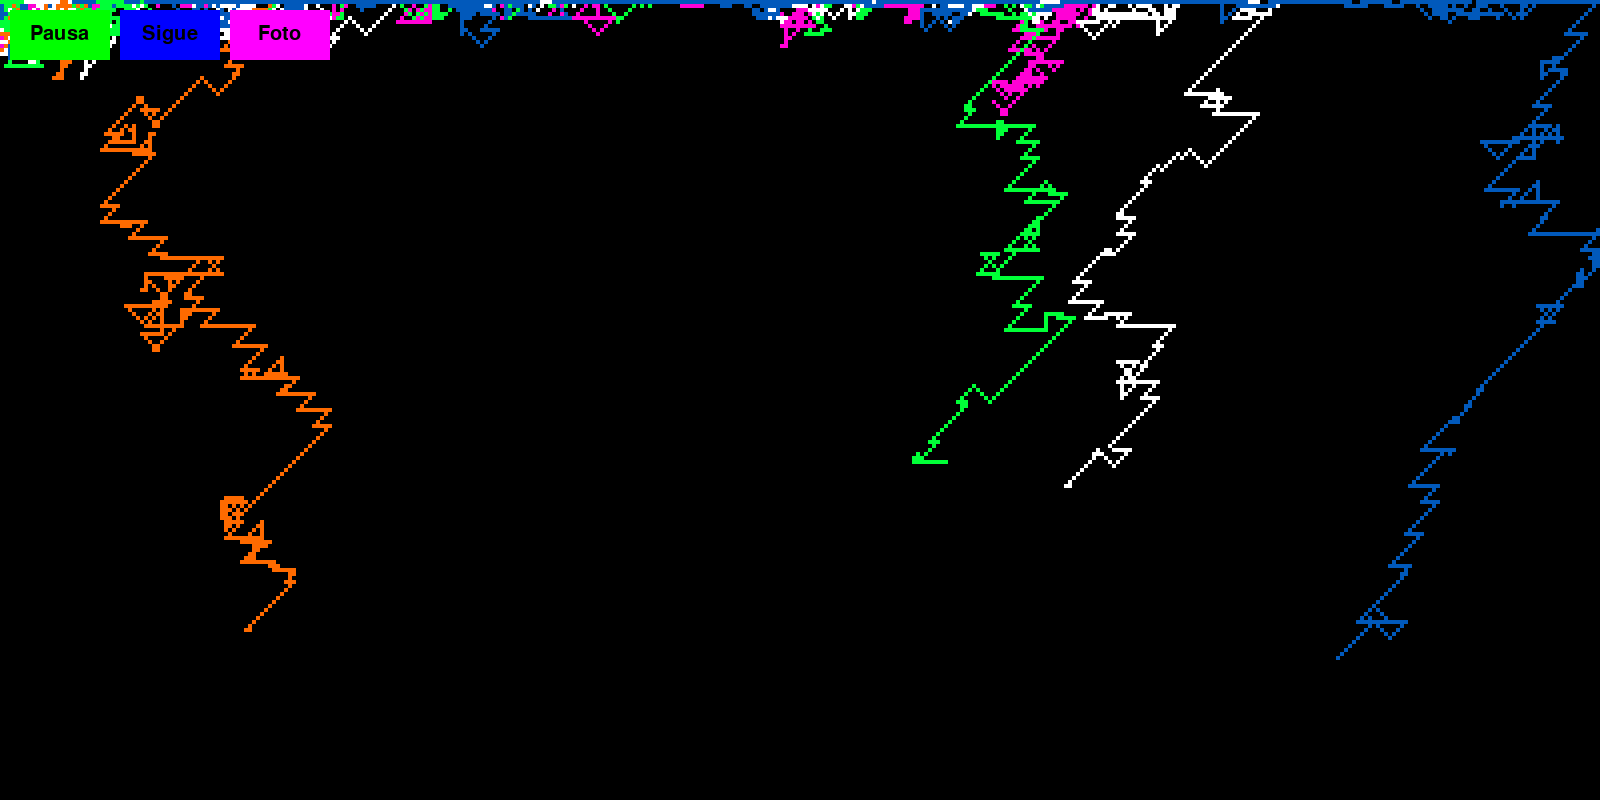
\includegraphics[width=\textwidth]{walkerNormal} % Asegúrate de cambiar la ruta a la ubicación de tu imagen
		\caption{Caminante Aleatorio con distribución normal}
	\end{figure}
\end{frame}

\begin{frame}
	\frametitle{Gamma - Normal}
	
	\begin{columns}
		
		% Columna de la izquierda
		\begin{column}{0.5\textwidth} % Ajusta la proporción según necesites
			\begin{figure}
				\centering
				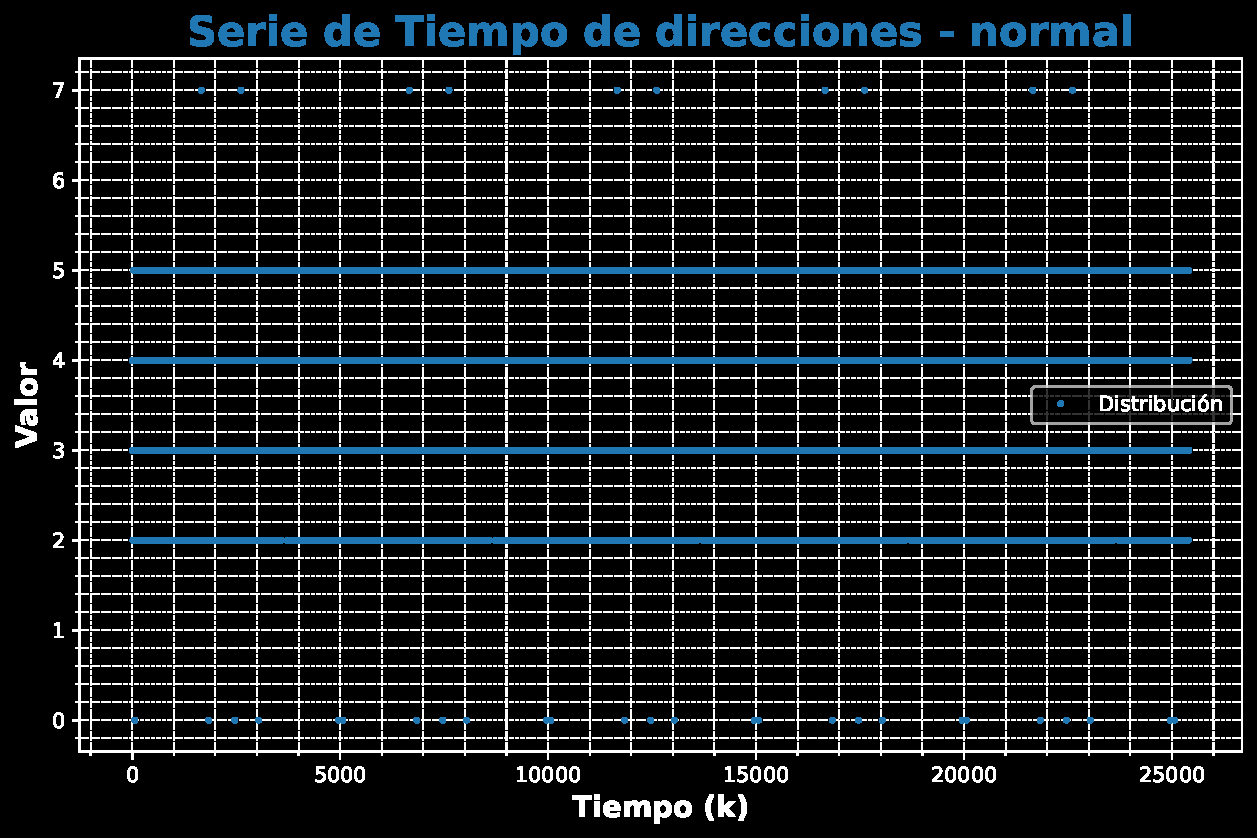
\includegraphics[width=\textwidth]{graf_direcciones_normal} % Asegúrate de cambiar la ruta a la ubicación de tu imagen
				\caption{Gráfica de la serie de tiempo para las direcciones.}
			\end{figure}
		\end{column}
		
		% Columna de la derecha
		\begin{column}{0.5\textwidth} % Ajusta la proporción según necesites
			\begin{figure}
				\centering
				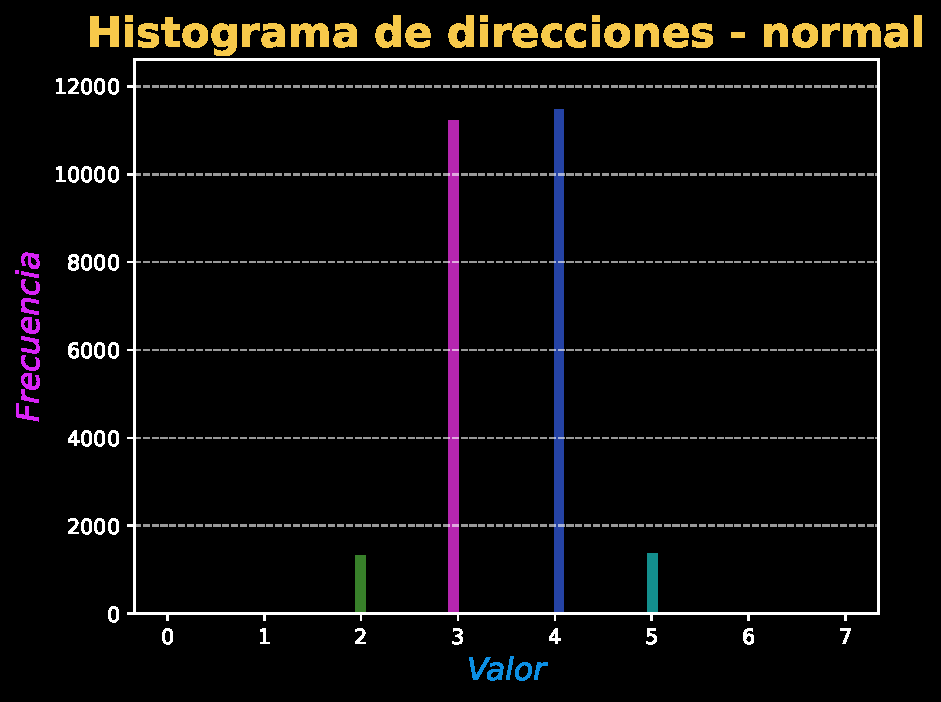
\includegraphics[width=\textwidth]{hist_direcciones_normal} % Asegúrate de cambiar la ruta a la ubicación de tu imagen
				\caption{Histograma de los datos de direcciones.}
			\end{figure}
		\end{column}
	\end{columns}
\end{frame}


\begin{frame}
	\frametitle{Caminante Aleatorio - Datos Gamma}
	\begin{figure}
		\centering
		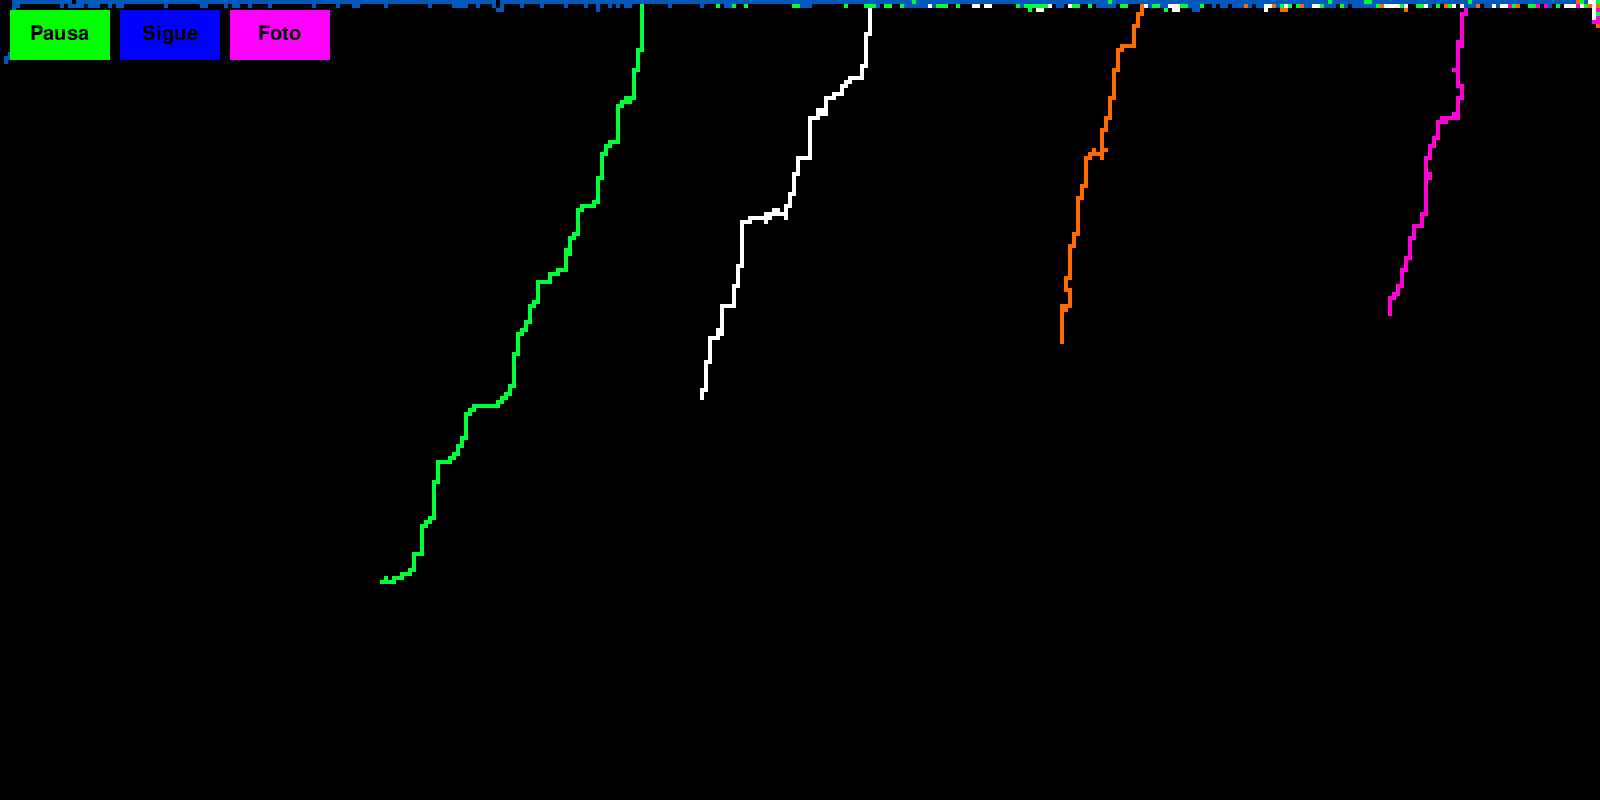
\includegraphics[width=\textwidth]{walkerGamma} % Asegúrate de cambiar la ruta a la ubicación de tu imagen
		\caption{Caminante Aleatorio con distribución gamma}
	\end{figure}
\end{frame}



\begin{frame}
	\frametitle{Gamma - Direcciones}
	
	\begin{columns}
		
		% Columna de la izquierda
		\begin{column}{0.5\textwidth} % Ajusta la proporción según necesites
			\begin{figure}
				\centering
				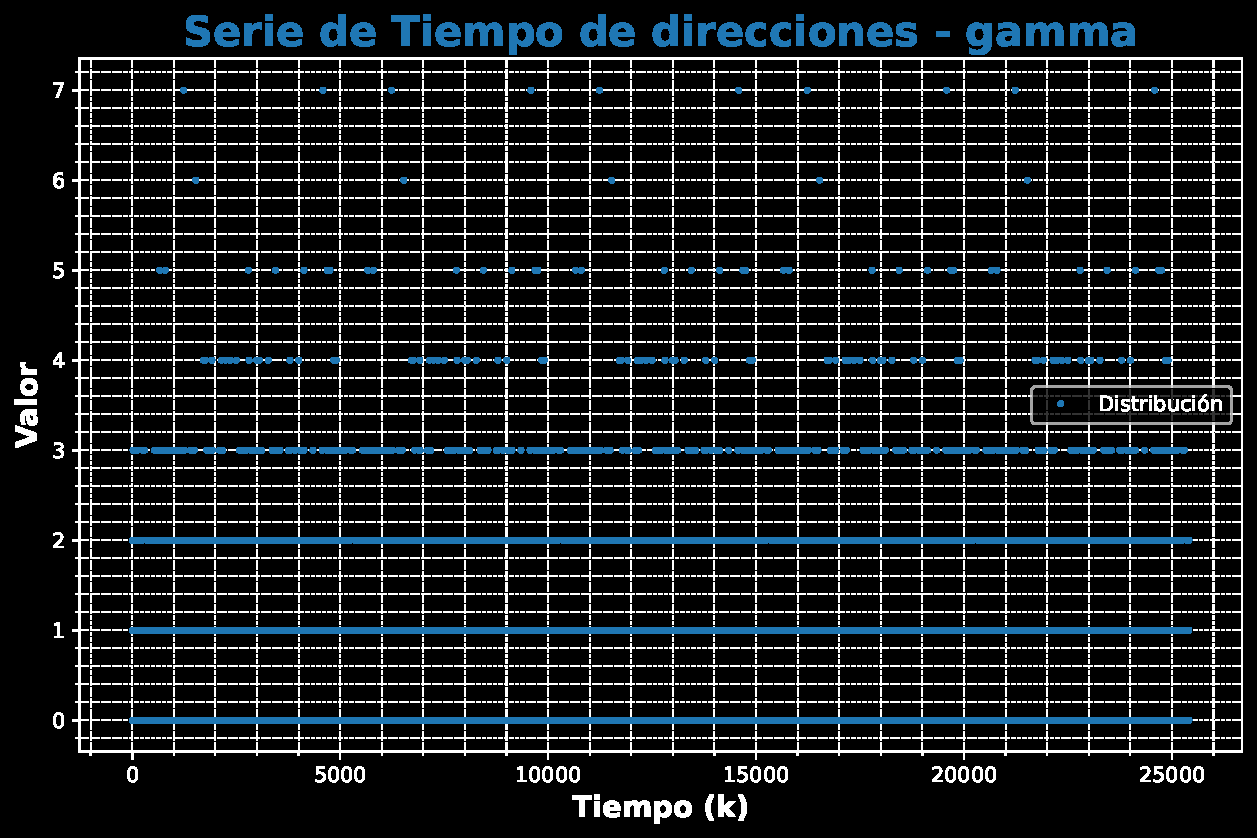
\includegraphics[width=\textwidth]{graf_direcciones_gamma} % Asegúrate de cambiar la ruta a la ubicación de tu imagen
				\caption{Gráfica de la serie de tiempo para las direcciones.}
			\end{figure}
		\end{column}
		
		% Columna de la derecha
		\begin{column}{0.5\textwidth} % Ajusta la proporción según necesites
			\begin{figure}
				\centering
				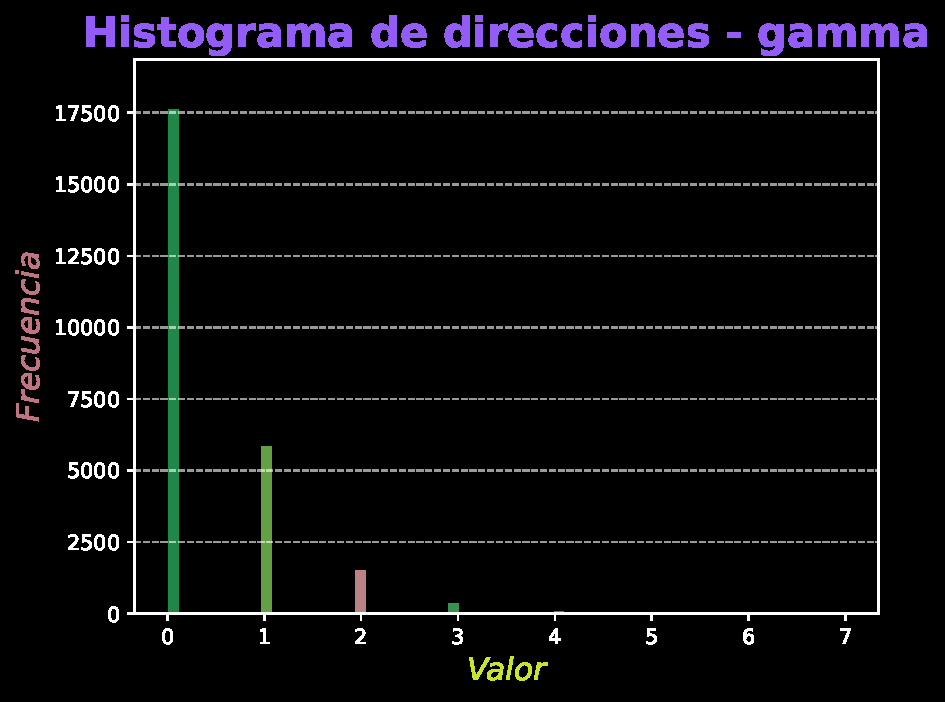
\includegraphics[width=\textwidth]{hist_direcciones_gamma} % Asegúrate de cambiar la ruta a la ubicación de tu imagen
				\caption{Histograma de los datos de direcciones.}
			\end{figure}
		\end{column}
	\end{columns}
\end{frame}